\documentclass{ctexart}
\ctexset{
proofname = \heiti{证明}
}
\usepackage{amsmath,amsthm,amsfonts,amssymb}
\usepackage{enumitem}
\usepackage{esdiff}
\usepackage{pifont}
\numberwithin{equation}{section}
\newtheorem{definition}{定义}
\newtheorem{thm}{定理}
\newtheorem{pro}{命题}
\newtheorem{cor}{推论}
\newtheorem{example}{例}
\newtheorem*{solution}{解}
\def\P{\textbf{P}}
\def\E{\mathbb{E}}
\def\Tr{\mathrm{Tr}}
\def\R{\mathbb{R}}
\def\Z{\mathcal{Z}}
\def\Var{\textrm{Var}}
\def\Cov{\textrm{Cov}}
\usepackage{mathtools}
\DeclareMathOperator*\argmin{\arg\!\min}
\DeclarePairedDelimiter\abs{\lvert}{\rvert}
\usepackage{bm}
\begin{document}
\title{波形估计理论}
\author{赵丰}
\maketitle
$z(t)$ 为观测,$s(t)$为待估计的信号波形,具体可分为三种类型:
\begin{enumerate}
\item 预测问题:$ g(t) = s(t+\alpha),\alpha>0 $
\item 滤波问题:$ g(t) = s(t)$
\item 平滑(内插)问题: $ g(t)=s(t), t\in $ 观测区间$I$。
\end{enumerate}

\section{波形的线性最小均方估计}
\subsection{线性最小均方估计}
寻找线性估值:$\hat{g}(t) = L[z(\xi)]$, 其中$L[\cdot]$为线性算子。使得 均方误差 $ e^2 = \E[(g(t)-\hat{g}(t))^2] $ 最小。
\begin{thm}
假设$L[z(\xi)]$ 满足正交性原理,即:
$\E[(g(t)-L[z(\xi)])z(\xi_i)]=0,\forall \xi_i \in I$
则对于另一线性算子 $L_1[\cdot]$,有:
\begin{equation}
\E[(g(t)-L[z(\xi)])^2]\leq \E[ (g(t)-L_1[z(\xi)])^2 ]
\end{equation}
\begin{proof}
\begin{align*}
\E[ (g(t)-L_1[z(\xi)])^2 ] & = \E[ (g(t)-L[z(\xi)]+L[z(\xi)]-L_1[z(\xi)])^2 ] \\
& = \E[ (g(t)-L[z(\xi)])^2 ] + \E[ (L[z(\xi)]-L_1[z(\xi)])^2 ] \\
& \geq \E[ (g(t)-L[z(\xi)])^2 ]
\end{align*}
\end{proof}
\end{thm}
\subsection{最佳线性滤波器}
设观测区间为 $ I = [0,T],$
$ \hat{g}(t) = \int_0^T h(t,\xi) z(\xi) d\xi $,
\begin{enumerate}
\item 由正交性原理:$\E[(g(t)-L[z(\xi)])z(\tau)]=0,\forall \tau \in [0,T]$
由此得到 Wiener-Hopf 方程: 
\begin{equation}\label{eq:WH}
R_{gz}(t,\tau) = \int_0^T h(t,\xi)R_z(\xi,\tau)d\xi,\tau \in [0,T]
\end{equation}
此时均方误差为
\begin{align}\notag 
e^2_{\min}  & =  \E[(g(t)- \int_0^T h(t,\xi)z(\xi)d\xi)g(t)] \\
 \label{eq:error}& = R_g(t,t) - \int_0^T h(t,\xi) R_{gz}(t,\xi)d\xi
\end{align}
\item 由变分法求解: 

希望求最佳的$h_1(t,\xi)$以使均方误差$ e^2 = \E[(g(t)-\int_0^T h_1(t,\xi)z(\xi)d\xi)^2]$ 最小,其中 $ h_1(t,\xi) = h(t,\xi) + \epsilon f(t,\xi) $,
$h(t,\xi)$ 是最优解,$\epsilon$ 是小的扰动因子, $f(t,\xi)$ 是扰动函数。
将均方误差重写为:$ e^2 = R_g(t,t)+\int_0^T\int_0^T h_1(t,\xi)h_1(t,\eta)R_z(\eta,\xi)d\eta d\xi -2\int_0^T h_1(t,\xi)R_{gz}(t,\xi)d\xi $.

令 $\diff{e^2(\epsilon)}{\epsilon}\bigg\rvert_{\epsilon=0} = 0 $  可得:
$ \int_0^T f(t,\epsilon)[R_{gz}(t,\xi) - \int_0^T h(t,\eta) R_z(\eta, \xi) d\eta ] d\xi = 0 $
由$f(t,\xi)$ 的任意性得:
$ R_{gz}(t,\xi) = \int_0^T h(t,\eta) R_z(\eta, \xi) d\eta,\xi\in [0,T]$
\end{enumerate}
\section{Wiener 滤波}
假定 $z(t)$ 平稳,$g(t)$ 与 $z(t)$ 联合平稳, 则 $R_{gz} (t, \tau) = R(t-\tau), R_z(t,\tau) = R_z(t-\tau)$, 并且设
$ h(t,\tau) = h(t - \tau)$,则 Wiener-Hopf 方程 式\eqref{eq:WH} 可改写为:
\begin{equation}\label{eq:stationary}
R_{gz}(t - \tau) = \int_0^T h(t - \xi)R_z(\xi - \tau)d\xi, \tau \in [0,T]
\end{equation}
由\eqref{eq:error} 可得其均方误差为:
\begin{equation}\label{eq:error_wiener}
    e^2_{\min} = R_g(0) - \int_0^T h(t-\xi) R_{gz}(t-\xi) d\xi
\end{equation}
\subsection{物理不可实现的 Wiener 滤波器}
将观测区间从$[0,T]$ 扩展到 $(-\infty, +\infty)$上,令$u = t - \tau, v = t - \xi, \xi - \tau = u - v  $
,则~(\ref{eq:stationary},\ref{eq:error_wiener})式可化为
\begin{align}
\label{eq:physical_impossible_wf} R_{gz} (u)  & = \int_{-\infty}^{+\infty} h(v) R_z(u - v)dv = h(u) * R_z(u) \\
\label{eq:error_wiener_pi}e^2_{\min}  & = R_g(0) - \int_{-\infty}^{+\infty} h(v) R_{gz}(v) dv
\end{align}
等式\eqref{eq:physical_impossible_wf} 右端为一卷积的形式, 作双边拉氏变换可得
\begin{equation}\label{eq:wf_pi_l}
\Phi_{gz} (\omega) = H(\omega) \Phi_z(\omega)
\end{equation}
做如下符号约定:
\begin{align*}
\hat{f}(\omega) & = \int_{\mathbb{R}} f(t)exp(-i\omega t) dt && \textrm{傅氏正变换}\\
f(t) & = {1 \over 2\pi}\int_{\mathbb{R}} \hat{f}(\omega)exp(i\omega t) d\omega && \textrm{傅氏反变换}\\
F(s) & = \int_{-\infty}^{+\infty} f(t)e^{-st}dt && \textrm{拉氏正变换}\\
f(t) & = {1 \over 2\pi i} \lim_{T \to \infty} \int_{\gamma - iT}^{\gamma + iT} e^{st} F(s)ds && \textrm{拉氏反变换}
\end{align*}
由相关函数是功率谱函数的Fourier反变换和Parseval定理,\eqref{eq:error_wiener_pi} 可化为
$$
e^2_{\min} = {1 \over 2\pi} \int_{-\infty}^{\infty} \Phi_g(\omega) d\omega - {1\over 2\pi} \int_{-\infty}^{\infty} H(\omega) \Phi^*_{gz}(\omega)d\omega
$$
由\eqref{eq:wf_pi_l}代入$H(\omega)$的表达式可得:
\begin{equation}\label{eq:wf_error_pi}
    e^2_{\min} = {1\over 2\pi} \int_{-\infty}^{+\infty} (\Phi_g(\omega) - {\abs{\Phi_{gz}(\omega)}^2 \over \Phi_z(\omega)}) d\omega
\end{equation}
\subsubsection{加性噪声}
$z(t) = s(t) + n(t)$, $s(t)$ 和 $n(t)$ 相互独立, $n(t)$ 的均值为零。
考虑滤波问题 $g(t) = s(t),$ 从而可得 $\Phi_{gz}(\omega) = \Phi_s(\omega)$, $\Phi_z(\omega) = \Phi_s(\omega) + \Phi_n(\omega)$,所以传输函数为:
$$
H(\omega) = \frac{\Phi_s(\omega)}{\Phi_s(\omega) + \Phi_n(\omega)}
$$
\begin{example}\label{ex:pi}
    已知 $\Phi_s(s) = \frac{2}{1-s^2}, \Phi_n(s) = 1$,求物理不可实现的 Wiener 滤波器的冲激响应 $h(t)$ 及其估值均方误差 $e^2_{\min}$。
    \begin{solution}
        $H(s) = \frac{2}{3 - s^2}$, 已知 $\mathcal{L}(e^{-\abs{t}}) = \frac{2}{1-s^2}$, 设$\mathcal{L}(f(t)) = F(s)$, 则 
        $\mathcal{L}(f(\alpha t)) = {1\over \alpha} F({s \over \alpha})$。 所以 
        $\mathcal{L}(e^{-\sqrt{3}\abs{t}}) = \sqrt{3} \frac{2}{3-s^2} \Rightarrow \mathcal{L}^{-1}(\frac{2}{3-s^2}) = \frac{1}{\sqrt{3}} 
        e^{-\sqrt{3}\abs{t}}$,由~\eqref{eq:wf_error_pi} 可得
        $$
        e^2_{\min} =  {1 \over 2\pi} \int_{-\infty}^{\infty} \frac{\Phi_s(\omega) \Phi_n(\omega)}{\Phi_s(\omega) + \Phi_n(\omega)} d\omega
        $$
        代入 $\Phi_s(\omega) = \frac{2}{1+\omega^2},\Phi_n(\omega) = 1$, 求得 $e^2_{\min} = \frac{1}{\sqrt{3}} = 0.577$.
    \end{solution}
\end{example}
\subsection{物理可实现的 Wiener 滤波器}
将观测区间由 $[0,T]$ 扩展到 $(-\infty, t)$, 仿照~(\ref{eq:physical_impossible_wf},\ref{eq:error_wiener_pi}) 式有:
\begin{align}
   \label{eq:physical_possible_wf} R_{gz}(u) & = \int_0^{+\infty} h(v)R_z(u-v)dv, u\geq 0 \\ 
   \label{eq:error_wiener_p} e^2_{\min} & = R_g(0) - \int_0^{+\infty} h(v) R_{gz}(v) dv
\end{align}
\subsubsection{频谱因式分解法}
将~\eqref{eq:physical_possible_wf} 扩展到$(-\infty,+\infty)$ 上, 引入 函数 $q(u)$
\begin{equation}\label{eq:wf_p_wp}
 \int_0^{+\infty} h(v)R_z(u-v)dv - R_{gz}(u) = q(u)
\end{equation}
满足 $ q(u) = 0, u \geq 0$, $Q(s) \triangleq \mathcal{L}(q(u))$ ,$Q(s)$的极点在$s$平面的右半平面。
同时补充定义 $h(v)=0, v<0$,则$H(s)$的极点在左半平面。

对~\eqref{eq:wf_p_wp} 作双边拉氏变换可得:
$ H(s)\Phi_z(s) - \Phi_{gz}(s)= Q(s) $。 假设 $R_z(\tau)$ 是实偶函数,则 $\Phi_z(s)$ 为有理谱($\Phi_z(j\omega)$ 为实数),于是$\Phi_z(s)$
可以分解为
\begin{equation} \label{eq:Phi_z_decom}    
\Phi_z(s) = \Phi_z^+(s)\Phi_z^{-}(s)
\end{equation} 
其中 $\Phi_z^+(s)$ 的零极点在左半平面, $\Phi_z^{-}(s) = \Phi_z^+(-s)$ 的零极点在右半平面。
从而可得 
\begin{equation}\label{eq:HPhi}
H(s) \Phi_z^+(s) = \frac{Q(s)}{\Phi_z^{-}(s)} + \frac{\Phi_{gz}(s)}{\Phi_z^{-}(s)}
\end{equation}
式~\eqref{eq:HPhi} 右端第二项可以通过部分分式分解为两部分之和:
$$
\frac{\Phi_{gz}(s)}{\Phi_z^{-}(s)} = \left[\frac{\Phi_{gz}(s)}{\Phi_z^{-}(s)}\right]^{t+} + \left[\frac{\Phi_{gz}(s)}{\Phi_z^{-}(s)}\right]^{t-}
$$
其中$[\cdot]^{t+}$ 的极点都在左半平面($t+$是指时域响应只在$t\geq 0$时有),而$[\cdot]^{t-}$ 的极点都在右半平面,同时含部分分式分解中的常数项,且这种
分解是唯一的。
假设 $H(s),\Phi_z(s)$ 分母阶次比分子高, 在等式~\eqref{eq:HPhi} 两端同时取 $[\cdot]^{t+}$ 可得:
$ H(s)\Phi_z^+(s) = [\frac{\Phi_{gz}(s)}{\Phi_z^{-}(s)}]^{t+} $
即 
\begin{equation}\label{eq:wiener_transfer_p}
H(s) = \frac{1}{\Phi_z^+(s)}\left[\frac{\Phi_{gz}(s)}{\Phi_z^{-}(s)}\right]^{t+}
\end{equation}
\subsubsection{预白化法}
若$z(t)$ 为白信号, 即 $R_z(\tau) = \delta(\tau)$, 由 Wiener-Hopf 方程 ~\eqref{eq:physical_possible_wf} 式得到:
\begin{equation}\label{eq:white_method_a}
h(t) = \begin{cases} R_{gz}(t), & t\geq 0 \\
    0, & t<0 \\
\end{cases}
\xleftrightarrow{\quad\mathcal{L}\quad} H(s) = [\Phi_{gz}(s)]^{t+}
\end{equation}
若 $z(t)$ 为非白信号, 则可先将 $z(t)$ 通过白化滤波器$H_W(s)$ 变成白信号 $x(t)$, 再对 $x(t)$ 采用滤波器 $H_2(s) = [\Phi_{gx}(s)]^{t+}$, 则
总的滤波器 $ H(s) = H_W(s) H_2(s)$ 就是我们要求的 Wiener 滤波器。

已知 输入的随机信号$ x(t) $ 通过 一个线性时不变系统(冲击响应为$h(t)$), 输出信号为$ y(t) $, 则 输入输出信号的PSD 满足 $ \Phi_y(s) = \Phi_x(s) H(s) H(-s) $

因此若使得 $\Phi_x(s) = 1 = \Phi_z(s) H_W(s) H_W(-s)$, 根据~\eqref{eq:Phi_z_decom} 式, 取 $H_W(s) = 1/\Phi_z^+(s)$ 即可。
\begin{align*}
R_{gx}(\tau) & = \E[g(t)x(t-\tau)] && = \E[g(t)\int_{-\infty}^{+\infty} h_W(\xi) z(t-\tau-\xi)d\xi] \\
& = \int_{-\infty}^{+\infty} h_W(\xi) R_{gz}(\tau + \xi)d\xi && = h_W(-\tau) * R_{gz}(\tau)
\end{align*}
所以 $ \Phi_{gx}(s) = H_W(-s) \Phi_{gz}(s) = \frac{\Phi_{gz}(s)}{\Phi_z^+(-s)} = \frac{\Phi_{gz}(s)}{\Phi_z^{-}(s)}$。
最终得到的滤波器即为~\eqref{eq:wiener_transfer_p} 所示。
\subsubsection{Wiener 滤波器的估值方差}
由~\eqref{eq:error_wiener_p} 式可以求出:
\begin{equation}\label{eq:wf_error_p}
    e^2_{\min} = R_g(0) - \int_0^{+\infty} R_{gx}^2(\tau) d\tau
\end{equation}
\begin{example}\label{ex:pi2}
沿用例~\ref{ex:pi},求物理可实现的 Wiener 滤波器 $h(t)$ 及其估值方差 $e^2_{\min}$
\begin{solution}
    \begin{align*}
    \Phi_z(s) & = \Phi_s(s) + \Phi_n(s) = \frac{3 - s^2}{1 - s^2} \\
    \Phi_z^+(s) & = \frac{\sqrt{3}+s}{1+s} \\
    \Phi_z^{-}(s) & = \frac{\sqrt{3} - s}{1 - s}    
    \end{align*}
    由于 $\Phi_{gz}(s) = \Phi_s(s) = \frac{2}{1 - s^2} $
    \begin{align*}
    \frac{\Phi_{gz}(s)}{\Phi_z^{-}(s)} & = \frac{\sqrt{3}-1}{1+s} + \frac{\sqrt{3}-1}{\sqrt{3}-s} \Rightarrow
    \left[\frac{\Phi_{gz}(s)}{\Phi_z^{-}(s)}\right]^{t+} = \frac{\sqrt{3}-1}{1+s} \\
    H(s) & = \frac{\sqrt{3}-1}{\sqrt{3}+s} \Rightarrow h(t) = (\sqrt{3} - 1) e^{-\sqrt{3} t} u(t)
    \end{align*}
    由双边拉氏反变换求得 $R_s(\tau) = e^{-\abs{\tau}} \Rightarrow R_s(0) = 1$ 
    $$
    \Phi_{gx}(s) = \frac{\Phi_{gz}(s)}{\Phi_z^{-}(s)} \Rightarrow R_{gx}(s) = (\sqrt{3}-1)e^{\sqrt{3} t} u(-t)+ (\sqrt{3}-1)e^{-t}u(t)
    $$
    代入~\eqref{eq:wf_error_p}式中求得:
    $ e^2_{\min} = \sqrt{3} - 1 = 0.732 $。
    由此可见: 物理可实现的$h(t)$ 的估值方差比物理不可实现的$h(t)$ 的估值方差要大。
    \begin{table}[!ht]
    \centering
    \begin{tabular}{cccc}
        \hline
        & $H(s)$ & $e^2_{\min}$ & $h(t)$  \\
        \hline
        物理不可实现 & ${2 \over 3-s^2}$ & ${1 \over \sqrt{3}}$ &$ {1 \over \sqrt{3} } \exp(-\sqrt{3} \abs{t} ) $ \\
        \hline
        物理可实现 & $ {\sqrt{3} - 1 \over \sqrt{3} + s} $ & $(\sqrt{3} - 1)$ & $ (\sqrt{3}-1)\exp(-\sqrt{3} t) u(t) $ \\
        \hline
    \end{tabular}
    \caption{例~\ref{ex:pi}、例~\ref{ex:pi2} 性能对比 }
    \end{table}
\end{solution}
\end{example}
\section{Kalman 滤波器}
\subsection{离散时间 Kalman 滤波}
已知状态方程:
\begin{equation}\label{eq:state}
X_k = \Phi_{k,k-1} X_{k-1} + W_{k-1}, k \geq 1
\end{equation}
观测方程: 
\begin{equation}\label{eq:observation}
Z_k = H_k X_k + V_k, k \geq 1
\end{equation}

其中
\begin{itemize}
\item $\Phi_{k, k-1}$ 是一步转移矩
\item $W_k$ 是动态噪声, 均值为0,协方差矩阵是 $ \Cov(W_k, W_i) = Q_k \delta_{ki} $;
\item $V_k $ 是观测噪声, 均值为0, 协方差矩阵是 $\Cov(V_k, V_i) = R_k \delta_{ki}$。
$W_k$ 和 $V_i$ 互不相关。
\item $H_k$ 是观测矩阵。
\item 初始状态 $X_0$ 均值为 $\mu_0$, 方差为 $P_0$, 与 $W_k, V_i$ 均不相关。
\end{itemize}
设计 $X_k$ 的线性估计器 $\hat{X}_k = \sum_{i=1}^k c_i Z_i$, 使得均方误差 $\E[\widetilde{X}_k^T \widetilde{X}_k]$ 最小, 其中 $\widetilde{X}_k = \hat{X}_k - X_k $。

采用直观推导的方法,
假设$\hat{X}_{k-1}$ 已经求出, 在没有新的观测的情况下,最佳一步预测为 
\begin{equation}\label{eq:single_step_predict}
\hat{X}_{k / k-1} =  \Phi_{k,k-1} \hat{X}_{k-1}
\end{equation}
当有新的观测$Z_k$ 时,
\begin{equation}\label{eq:state_estimate}
\hat{X}_k = \hat{X}_{k / k-1}  + K_k (Z_k - H_k \hat{X}_{k / k-1})
\end{equation}
希望优化Kalman 增益矩阵 $K_k$ 使得$\E[\widetilde{X}_k^T \widetilde{X}_k]$ 最小, 其中
$ \widetilde{X}_k = \hat{X}_k - X_k$ 。

代入观测方程~\eqref{eq:observation} 式有
\begin{align}
\widetilde{X}_k  & =  (\hat{X}_{k/k-1} - X_k) + K_k ( H_k X_k + V_k - H_k \hat{X}_{k/k-1} \nonumber\\
& = (I- K_k H_k)\widetilde{X}_{k/k-1} +K_k V_k \nonumber
\end{align}
其中 $\widetilde{X}_{k/k-1} = \hat{X}_{k/k-1} - X_k $, 代入一步预测方程~\eqref{eq:single_step_predict} 和状态方程 ~\eqref{eq:state} 可得
\begin{align*}
\widetilde{X}_{k/k-1}  & = \Phi_{k-1,k} \hat{X}_{k-1} - (\Phi_{k-1,k} X_{k-1} + W_{k-1} )\\
& = \Phi_{k-1, k} \widetilde{X}_{k-1} - W_{k-1}
\end{align*}

因为$\E[\widetilde{X}_k^T \widetilde{X}_k]  = \Tr[P_k]$,
记 $P_k = \E[\widetilde{X}_k \widetilde{X}_k^T] $, 为估计误差的方差矩阵。
记 $P_{k/k-1} = \E[\widetilde{X}_{k/k-1}\widetilde{X}_{k/k-1}^T] $ 为一步向前预测估值的方差矩阵,则
\begin{align}
P_k  & = (I- K_k H_k)P_{k/k-1} (I- K_k H_k)^T+K_k R_k K_k^T  \nonumber \\
P_{k/k-1} & = \Phi_{k-1, k} P_{k-1} \Phi_{k-1, k}^T + Q_{k-1} \label{covariance_predict}
\end{align}
$P_k$ 是关于 $K_k$的二次型矩阵函数,可采用“配平方” 法求“最小值”,从而有
\begin{align*}
P_k & = [K_k - P_{k/k-1} H_k^T (H_k P_{k/k-1} H_k^T + R_k)^{-1} ] (H_k P_{k/k-1} H_k^T + R_k) \\
&[K_k - P_{k/k-1} H_k^T (H_k P_{k/k-1} H_k^T + R_k)^{-1} ]^T + P_{k/k-1} - P_{k/k-1} H_k^T(H_k P_{k/k-1} H_k^T + R_k)^{-1}
H_k P_{k/k-1}^T
\end{align*}
因此取
\begin{equation}\label{eq:gain_update}
 K_k = P_{k/k-1} H_k^T(H_k P_{k/k-1} H_k^T + R_k)^{-1}
 \end{equation}
 $P_k$ 最小,最小值为
\begin{equation}\label{eq:covariance_update}
P_k = (I - K_k H_k)P_{k/k-1}
\end{equation}

在实际操作中,通常按照 ~\eqref{eq:single_step_predict}, ~\eqref{covariance_predict}, ~\eqref{eq:gain_update},
~\eqref{eq:state_estimate},
~\eqref{eq:covariance_update}
五个公式顺序迭代求解。

\begin{example}[地面雷达对空中目标的跟踪]
  如果雷达站到目标的斜距为 $x(t)$,其变化率 $ \dot{x}(t)$ 为常数。
  从 $ t = 0 $ 时, 开始观测目标,观测间隔为 1 秒, 测得 $ x(t)$ 的四个观测值为:
  $ z(1) = 1.1km, z(2)  = 2.0km, z(3) = 3.2km, z(4) = 3.8km $。
  已知:$ \E[x(0)] = 0, \E[\dot x(0)] = 0, \E[ x(0) \dot x(0)] = 0, \E[ x^2(0) ] = 10 km^2, \E [ \dot x^2(0) ] = 10 (km/s)^2,
  \E[ v(k) ] = 0, R(k) = 0.1 km^2 $。
  利用 Kalman 滤波的方法求斜距$x(t)$ 的最佳滤波值与滤波误差的方差。
\end{example}
\begin{solution}
设 $ \bm{x}_k = \begin{bmatrix} x(k) \\ \dot x(k) \end{bmatrix} $,
在状态方程~\eqref{eq:state}式中,$ \Phi = \begin{bmatrix} 1 & 1 \\ 0 & 1 \end{bmatrix} , Q = \bm{0}$;在观测方程
~\eqref{eq:observation}中, $ H = [1,0], V = 0.1 $。初始状态
$ \bm{x}_0 = \begin{bmatrix} 0 \\ 0 \end{bmatrix},  P_0 = \begin{bmatrix} 10 & 0 \\ 0 & 10 \end{bmatrix} $。
按照 ~\eqref{eq:single_step_predict}, ~\eqref{covariance_predict}, ~\eqref{eq:gain_update},
~\eqref{eq:state_estimate},
~\eqref{eq:covariance_update}
得到估值如表~\ref{tab:lkf} 所示。

\begin{table}[!ht]
\centering
\begin{tabular}{|c|c|c|c|c|}
\hline
 $k$ & 1 & 2 & 3 & 4 \\
 \hline
 $\hat{x}(k)$ & 1.09 & 1.99 & 3.14 & 3.92 \\
 \hline
 $ \hat{\dot x}(k)$ & 0.55 & 0.89 & 1.04 & 0.93 \\
 \hline
\end{tabular}
\caption{Kalman 滤波估值}\label{tab:lkf}
\end{table}

估值方差变化情况如图~\ref{fig:lkf} 所示。

\begin{figure}
\centering
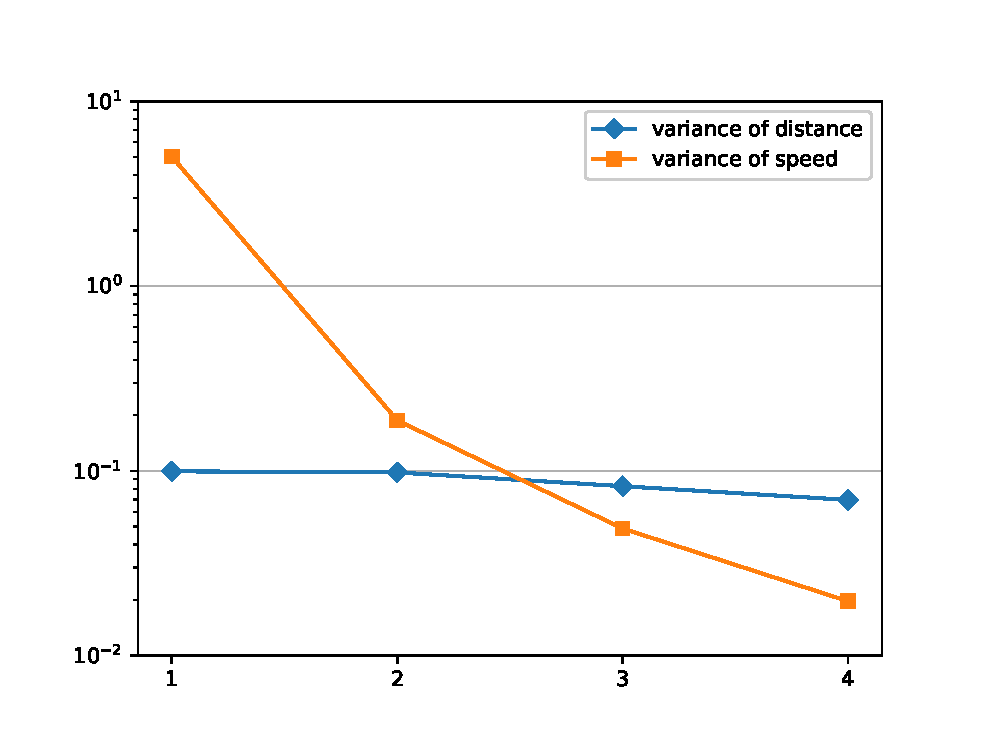
\includegraphics[width = 7cm]{kalman.eps}
\caption{Kalman 滤波估值方差}\label{fig:lkf}
\end{figure}
\end{solution}


\end{document}


